% From Ideas to Action: Napoleon, Berthier, and Lannes
% Compile with XeLaTeX:  latexmk -xelatex napoleon_berthier_lannes_v2.tex
\documentclass[aspectratio=169,10pt,t]{beamer}

% ---------------------------------------------------------------- fonts
\usefonttheme{professionalfonts}
\usepackage{fontspec}
\usepackage{unicode-math}
\setsansfont{Avenir Next}[
  UprightFont    = * Regular,
  BoldFont       = * Demi Bold,
  ItalicFont     = * Italic,
  BoldItalicFont = * Demi Bold Italic]
\newfontfamily\heavyfont{Avenir Next}[UprightFont = * Bold]
\setmathfont{STIX Two Math}[Scale=1.02]

\usepackage{booktabs,mathtools,tikz}
\usepackage{etoolbox}
\appto\normalsize{\setlength{\abovedisplayskip}{5pt}\setlength{\belowdisplayskip}{5pt}\setlength{\abovedisplayshortskip}{3pt}\setlength{\belowdisplayshortskip}{3pt}}
\appto\small{\setlength{\abovedisplayskip}{4pt}\setlength{\belowdisplayskip}{4pt}}
\usetikzlibrary{arrows.meta,positioning,calc,decorations.pathreplacing}

% --------------------------------------------------------------- colours
\definecolor{navy}{HTML}{14213D}
\definecolor{ink}{HTML}{1F2933}
\definecolor{muted}{HTML}{66717F}
\definecolor{hair}{HTML}{D5DAE1}
\definecolor{nap}{HTML}{B26B12}
\definecolor{ber}{HTML}{2C5FA8}
\definecolor{lan}{HTML}{23795A}
\definecolor{err}{HTML}{B0473A}

% ---------------------------------------------------------- beamer theme
\setbeamertemplate{navigation symbols}{}
\setbeamercolor{normal text}{fg=ink,bg=white}
\setbeamercolor{structure}{fg=navy}
\setbeamercolor{alerted text}{fg=err}
\setbeamertemplate{itemize items}{\raisebox{0.18em}{\color{navy}\rule{0.32em}{0.32em}}}
\setbeamertemplate{enumerate item}{\color{navy}\bfseries\insertenumlabel.}
\setlength{\leftmargini}{1.1em}
\setbeamersize{text margin left=1.0cm,text margin right=1.0cm}
\linespread{0.95}

% Kicker (small uppercase label) + assertion headline + hairline.
% Call \kicker{...} immediately before \begin{frame}.
\newcommand{\kicker}[1]{\gdef\insertkicker{#1}}
\def\insertkicker{}
\setbeamertemplate{frametitle}{%
  \vspace*{0.36cm}%
  \ifx\insertkicker\empty\else
    {\fontsize{7.5}{9}\selectfont\bfseries\color{muted}\addfontfeature{LetterSpace=8}\MakeUppercase{\insertkicker}}\par\vspace{0.1cm}%
  \fi
  {\fontsize{15.5}{18.5}\selectfont\bfseries\color{navy}\insertframetitle}\par
  \vspace{0.12cm}{\color{hair}\rule{\linewidth}{0.4pt}}%
  \global\let\insertkicker\empty
}

\newif\ifappendix
\setbeamertemplate{footline}{%
  \hbox to \paperwidth{\hspace{1.0cm}%
    {\fontsize{7}{8}\selectfont\color{muted}From Ideas to Action\enspace\textcolor{hair}{|}\enspace Napoleon $\cdot$ Berthier $\cdot$ Lannes}%
    \hfill
    {\fontsize{7}{8}\selectfont\color{muted}\ifappendix Appendix\enspace\fi\insertframenumber}%
    \hspace{1.0cm}}%
  \vspace{0.38cm}}

% ------------------------------------------------------------ components
\newsavebox{\cardsave}
% card{width}{colour}: soft-tinted panel with a coloured left rule
\newenvironment{card}[2]{%
  \def\cardcolor{#2}%
  \begin{lrbox}{\cardsave}\begin{minipage}{\dimexpr#1-26pt\relax}\raggedright}
  {\end{minipage}\end{lrbox}%
  \begin{tikzpicture}[baseline=(c.north)]
    \node[inner xsep=13pt,inner ysep=8pt,fill=\cardcolor!7,anchor=north west](c){\usebox{\cardsave}};
    \fill[\cardcolor](c.north west) rectangle ([xshift=2.4pt]c.south west);
  \end{tikzpicture}\par}
% cardh{width}{height}{colour}: same, fixed height for side-by-side panels
\newenvironment{cardh}[3]{%
  \def\cardcolor{#3}%
  \begin{lrbox}{\cardsave}\begin{minipage}[t][#2][t]{\dimexpr#1-26pt\relax}\raggedright}
  {\end{minipage}\end{lrbox}%
  \begin{tikzpicture}[baseline=(c.north)]
    \node[inner xsep=13pt,inner ysep=8pt,fill=\cardcolor!7,anchor=north west](c){\usebox{\cardsave}};
    \fill[\cardcolor](c.north west) rectangle ([xshift=2.4pt]c.south west);
  \end{tikzpicture}\par}
\tikzset{
  box/.style={minimum width=1.85cm,minimum height=1.15cm,align=center,fill=#1!8,draw=#1!55,line width=0.6pt},
  brace/.style={decorate,decoration={brace,mirror,amplitude=4pt},line width=0.6pt,#1}}
\newcommand{\cardtitle}[2]{{\fontsize{7.5}{9}\selectfont\bfseries\color{#2}\addfontfeature{LetterSpace=6}\MakeUppercase{#1}}\par\vspace{0.1cm}}
\newcommand{\smallnote}[1]{{\fontsize{7.5}{10}\selectfont\color{muted}#1\par}}
\newcommand{\role}[2]{\textcolor{#2}{\bfseries #1}}
\newcommand{\Nap}{\role{Napoleon}{nap}}
\newcommand{\Ber}{\role{Berthier}{ber}}
\newcommand{\Lan}{\role{Lannes}{lan}}

\newcommand{\E}{\mathbb{E}}
\DeclareMathOperator{\tr}{tr}
\DeclareMathOperator{\Var}{Var}
\DeclareMathOperator{\Cov}{Cov}
\newcommand{\Ycal}{\mathcal{Y}}
% labelled bracket under a term
\newcommand{\ub}[2]{\underset{\mathclap{\text{\fontsize{6.5}{7}\selectfont\color{muted}#2}}}{\underline{#1}}}

\title{From Ideas to Action}
\subtitle{Napoleon, Berthier, and Lannes}
\date{October 2026}

\begin{document}

% ======================================================================= 1
{\setbeamercolor{background canvas}{bg=navy}
\setbeamertemplate{footline}{}
\begin{frame}[plain,c]
  {\fontsize{8.5}{10}\selectfont\bfseries\color{nap!70!white}\addfontfeature{LetterSpace=10}A THEORY OF INTELLIGENCE AND PRODUCTION}\par
  \vspace{0.45cm}
  {\heavyfont\fontsize{38}{40}\selectfont\color{white}From Ideas to Action}\par
  \vspace{0.3cm}
  {\fontsize{15}{18}\selectfont\color{white!72!navy}Napoleon, Berthier, and Lannes}\par
  \vspace{1.0cm}
  
\begin{tikzpicture}[
      stage/.style={minimum width=3.65cm,minimum height=1.25cm,align=left,inner xsep=10pt,anchor=west,fill=white!7!navy},
      arr/.style={-{Stealth[length=5pt]},white!45!navy,line width=0.8pt}]
    \node[stage](n) at (0,0) {{\fontsize{8}{9}\selectfont\bfseries\color{nap!75!white}\addfontfeature{LetterSpace=6}NAPOLEON}\\[1pt]{\small\color{white}Conceive \& select ideas}};
    \node[stage](b) at (4.35,0) {{\fontsize{8}{9}\selectfont\bfseries\color{ber!45!white}\addfontfeature{LetterSpace=6}BERTHIER}\\[1pt]{\small\color{white}Formulate \& plan}};
    \node[stage](l) at (8.7,0) {{\fontsize{8}{9}\selectfont\bfseries\color{lan!50!white}\addfontfeature{LetterSpace=6}LANNES}\\[1pt]{\small\color{white}Execute physically}};
    \fill[nap!75!white] (n.north west) rectangle ([xshift=2.4pt]n.south west);
    \fill[ber!45!white] (b.north west) rectangle ([xshift=2.4pt]b.south west);
    \fill[lan!50!white] (l.north west) rectangle ([xshift=2.4pt]l.south west);
    \draw[arr] (n.east) -- (b.west);
    \draw[arr] (b.east) -- (l.west);
  \end{tikzpicture}\par
  \vspace{1.0cm}
  {\fontsize{8}{10}\selectfont\color{white!60!navy}Research model\enspace|\enspace October 2026}\par
\end{frame}}

% ======================================================================= 2
\kicker{Motivation}
\begin{frame}{Where will AI's economic value come from?}
  \vspace{0.3cm}
  \begin{columns}[T,onlytextwidth]
    \column{0.48\textwidth}
    \begin{cardh}{\linewidth}{2.0cm}{nap}
      \cardtitle{View 1 \textperiodcentered{} Better ideas}{nap}
      AI generates and selects ideas that humans would not have conceived.\par\vspace{0.15cm}
      \smallnote{Value comes from shifting the frontier of what is worth trying.}
    \end{cardh}
    \column{0.48\textwidth}
    \begin{cardh}{\linewidth}{2.0cm}{ber}
      \cardtitle{View 2 \textperiodcentered{} Better realization}{ber}
      AI makes the existing stock of human ideas faster and cheaper to turn into workable plans.\par\vspace{0.15cm}
      \smallnote{Value comes from closing the gap between an idea and its best plan.}
    \end{cardh}
  \end{columns}
  \vspace{0.55cm}
  This deck builds a production model that separates the two views, and adds the stage neither view controls: \textbf{physical execution}, which may bound throughput however good the thinking upstream.
\end{frame}

% ======================================================================= 3
\kicker{The hypothesis}
\begin{frame}{Intelligence is not a single factor of production}
  \vspace{0.3cm}
  \begin{columns}[T,onlytextwidth]
    \column{0.315\textwidth}
    \begin{cardh}{\linewidth}{2.45cm}{nap}\small
      \cardtitle{Napoleon}{nap}
      {\bfseries Conception}\par
      {\color{muted}What is worth trying?}\par\vspace{0.18cm}
      Produces and evaluates a vague idea $\xi$.
    \end{cardh}
    \column{0.315\textwidth}
    \begin{cardh}{\linewidth}{2.45cm}{ber}\small
      \cardtitle{Berthier}{ber}
      {\bfseries Mental execution}\par
      {\color{muted}What plan implements it?}\par\vspace{0.18cm}
      Formulates the problem and finds a \emph{fallible} plan $\hat a$.
    \end{cardh}
    \column{0.315\textwidth}
    \begin{cardh}{\linewidth}{2.45cm}{lan}\small
      \cardtitle{Lannes}{lan}
      {\bfseries Physical execution}\par
      {\color{muted}What actually happens?}\par\vspace{0.18cm}
      Carries out the plan, possibly imperfectly: $\tilde a$.
    \end{cardh}
  \end{columns}
  \vspace{0.35cm}
  \begin{card}{\linewidth}{navy}
    \textbf{Working hypothesis.} Current AI chiefly improves \Ber{}; an ASI would also be an exceptional \Nap{}. \Lan{} remains necessary whenever output requires physical action.
  \end{card}
\end{frame}

% ======================================================================= 4
\kicker{The project pipeline}
\begin{frame}{An idea is not a plan; a plan is not an outcome}
  \vspace{0.45cm}
  \centering
  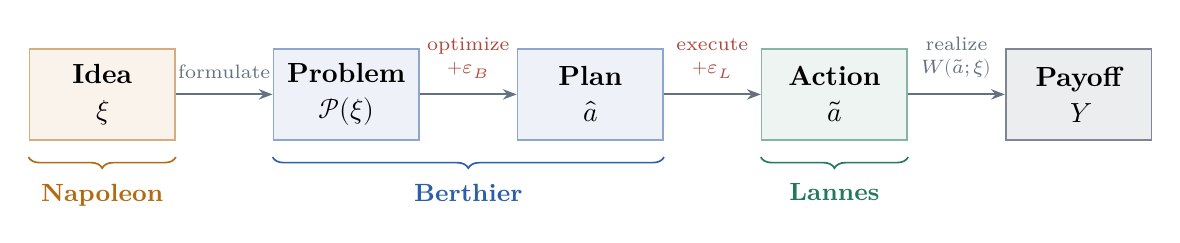
\begin{tikzpicture}[
      arr/.style={-{Stealth[length=5pt]},muted,line width=0.7pt},
      lab/.style={font=\fontsize{7}{8.5}\selectfont,color=muted,above=2pt,align=center}]
    \node[box=nap](i) at (0,0)    {\textbf{Idea}\\[1pt]$\xi$};
    \node[box=ber](p) at (3.1,0)  {\textbf{Problem}\\[1pt]$\mathcal{P}(\xi)$};
    \node[box=ber](a) at (6.2,0)  {\textbf{Plan}\\[1pt]$\hat a$};
    \node[box=lan](x) at (9.3,0)  {\textbf{Action}\\[1pt]$\tilde a$};
    \node[box=navy](y) at (12.4,0){\textbf{Payoff}\\[1pt]$Y$};
    \draw[arr] (i) -- node[lab]{formulate} (p);
    \draw[arr] (p) -- node[lab,text=err]{optimize\\$+\varepsilon_B$} (a);
    \draw[arr] (a) -- node[lab,text=err]{execute\\$+\varepsilon_L$} (x);
    \draw[arr] (x) -- node[lab]{realize\\$W(\tilde a;\xi)$} (y);
    \draw[brace=nap] ([yshift=-6pt]i.south west) -- ([yshift=-6pt]i.south east) node[midway,below=6pt,font=\small\bfseries,text=nap]{Napoleon};
    \draw[brace=ber] ([yshift=-6pt]p.south west) -- ([yshift=-6pt]a.south east) node[midway,below=6pt,font=\small\bfseries,text=ber]{Berthier};
    \draw[brace=lan] ([yshift=-6pt]x.south west) -- ([yshift=-6pt]x.south east) node[midway,below=6pt,font=\small\bfseries,text=lan]{Lannes};
  \end{tikzpicture}\par
  \raggedright
  \vspace{0.45cm}
  \begin{card}{\linewidth}{navy}
    An idea $\xi$ specifies a desired possibility. \Ber{} converts it into a well-defined problem, finds a plan, and hands the plan to \Lan{}. The resulting physical action generates payoff $Y$. Errors enter at planning ($\varepsilon_B$) and at execution ($\varepsilon_L$).
  \end{card}
\end{frame}

% ======================================================================= 5
\kicker{Stage 1 \textperiodcentered{} Idea search and selection}
\begin{frame}{Napoleon creates the variation across projects}
  \vspace{0.3cm}
  \begin{columns}[T,onlytextwidth]
    \column{0.5\textwidth}
    \begin{cardh}{\linewidth}{3.4cm}{nap}\small
      \cardtitle{Idea-generating technology}{nap}
      \[\xi_i \overset{\text{i.i.d.}}{\sim} F_A, \qquad \lambda_A = \frac{n_A}{\tau_A}\]
      \begin{itemize}\setlength{\itemsep}{1pt}
        \item One idea per Napoleon every $\tau_A$.
        \item $n_A$ Napoleons work in parallel.
        \item $F_A$ governs the \emph{quality} of ideas, not just their number.
      \end{itemize}
    \end{cardh}
    \column{0.45\textwidth}
    \cardtitle{Value of an idea}{navy}
    The value achievable with an optimal plan and perfect execution:
    \[v(\xi) = \max_{a\in\mathcal{A}(\xi)} W(a;\xi)\]
    In the baseline, Napoleon observes $v(\xi)$ and decides whether the idea deserves downstream capacity.
  \end{columns}
  \vspace{0.3cm}
  \smallnote{Progress at this stage can raise the arrival rate $\lambda_A$, shift the distribution of $v(\xi)$ upward, or sharpen Napoleon's ability to recognize valuable ideas.}
\end{frame}

% ======================================================================= 6
\kicker{Stage 2 \textperiodcentered{} Formulation and optimization}
\begin{frame}{Berthier turns a vague idea into a fallible plan}
  \begin{card}{\linewidth}{ber}
    \cardtitle{The benchmark problem induced by an idea}{ber}
    \vspace{-0.25cm}
    \[\mathcal{P}(\xi):\quad \max_{a\in\mathcal{A}(\xi)} W(a;\xi), \qquad a^*(\xi)\in\arg\max_{a\in\mathcal{A}(\xi)} W(a;\xi)\]
    \vspace{-0.15cm}
    \[\boxed{\;\hat a = a^*(\xi) + \varepsilon_B\;}\qquad \E[\varepsilon_B\mid\xi]=0,\quad \Var(\varepsilon_B\mid\xi)=\Omega_B\]
    \vspace{-0.2cm}
  \end{card}
  \vspace{0.3cm}
  \begin{columns}[T,onlytextwidth]
    \column{0.31\textwidth}
    \cardtitle{Formulation}{navy}
    {\small Translate a vague objective into decision variables, constraints, and payoffs.}
    \column{0.31\textwidth}
    \cardtitle{Optimization}{navy}
    {\small Spend scarce planning time $\tau_B$ searching for a good solution.}
    \column{0.31\textwidth}
    \cardtitle{What AI changes}{ber}
    {\small A better Berthier lowers $\Omega_B$, $\tau_B$, or both.}
  \end{columns}
  \vspace{0.2cm}
  \smallnote{$\varepsilon_B$ pools formulation and solution errors; a systematic formulation mistake would add bias (Appendix A2).}
\end{frame}

% ======================================================================= 7
\kicker{Stage 3 \textperiodcentered{} Execution}
\begin{frame}{A correct plan does not guarantee correct execution}
  \vspace{0.25cm}
  \begin{card}{\linewidth}{lan}
    \vspace{-0.3cm}
    \[\boxed{\;\tilde a = \hat a + \varepsilon_L\;}\qquad \E[\varepsilon_L\mid\xi,\varepsilon_B]=0,\quad \Var(\varepsilon_L\mid\xi)=\Omega_L\]
    \vspace{-0.3cm}
  \end{card}
  \vspace{0.45cm}
  \centering
  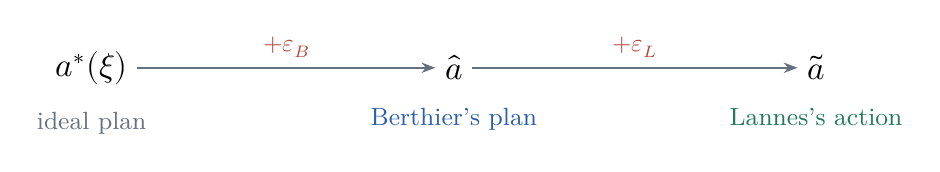
\begin{tikzpicture}[arr/.style={-{Stealth[length=5pt]},muted,line width=0.7pt},
                      capt/.style={font=\small,below=3pt}]
    \node(s) at (0,0) {\large$a^*(\xi)$};
    \node(h) at (4.6,0) {\large$\hat a$};
    \node(t) at (9.2,0) {\large$\tilde a$};
    \draw[arr] (s) -- node[above,font=\small,text=err]{$+\varepsilon_B$} (h);
    \draw[arr] (h) -- node[above,font=\small,text=err]{$+\varepsilon_L$} (t);
    \node[capt,text=muted] at (s.south) {ideal plan};
    \node[capt,text=ber] at (h.south) {Berthier's plan};
    \node[capt,text=lan] at (t.south) {Lannes's action};
  \end{tikzpicture}\par
  \raggedright
  \vspace{0.35cm}
  \textbf{Sources of $\varepsilon_L$:} late arrival, miscommunication, local friction, inaccurate maneuvering, or inability to supply the commanded effort.\par
  \vspace{0.25cm}
  \smallnote{A single realization of $\varepsilon_L$ may happen to offset Berthier's mistake; the model guarantees losses only in expectation.}
\end{frame}

% ======================================================================= 8
\kicker{Payoff technology}
\begin{frame}{Planning and execution losses enter additively}
  \vspace{0.15cm}
  \cardtitle{Quadratic loss around the ideal plan}{navy}
  \vspace{-0.3cm}
  \[W(a;\xi) = v(\xi) - \tfrac12\big(a-a^*(\xi)\big)^{\!\top} H\big(a-a^*(\xi)\big),\qquad H\succ 0,\qquad Y(\xi)=W(\tilde a;\xi)\]
  \par\vspace{0.05cm}
  \mbox{}The realized deviation is $\varepsilon_B+\varepsilon_L$. With mean-zero, independent errors, the cross term vanishes:\par
  \vspace{0.1cm}
  \begin{card}{\linewidth}{navy}
    \vspace{-0.3cm}
    \[\E[Y\mid\xi] \;=\; v(\xi) \;-\; \ub{\tfrac12\tr(H\Omega_B)}{\color{ber}$\kappa_B$: planning loss} \;-\; \ub{\tfrac12\tr(H\Omega_L)}{\color{lan}$\kappa_L$: execution loss}\]
  \end{card}
  \vspace{0.3cm}
  \smallnote{Baseline: $H$, $\Omega_B$, and $\Omega_L$ do not depend on $\xi$, so ideas can be ranked by $v(\xi)$ alone.}
\end{frame}

% ======================================================================= 9
\kicker{Capacity}
\begin{frame}{The slower downstream stage caps throughput}
  \vspace{0.15cm}
  \centering
  \renewcommand{\arraystretch}{1.2}
  \begin{tabular}{@{}l c c c@{}}
    \toprule
    \textbf{Stage} & \textbf{Workers} & \textbf{Time per project} & \textbf{Rate} \\
    \midrule
    \Nap{}: ideas   & $n_A$ & $\tau_A$ & $\lambda_A = n_A/\tau_A$ \\
    \Ber{}: plans   & $n_B$ & $\tau_B$ & $\mu_B = n_B/\tau_B$ \\
    \Lan{}: actions & $n_L$ & $\tau_L$ & $\mu_L = n_L/\tau_L$ \\
    \bottomrule
  \end{tabular}\par
  \raggedright
  \vspace{0.3cm}
  \begin{card}{\linewidth}{navy}
    With a sufficient supply of accepted ideas, long-run throughput is bounded by downstream capacity:
    \vspace{-0.15cm}
    \[\boxed{\;K=\min\{\mu_B,\ \mu_L\}\;}\]
    \vspace{-0.3cm}
  \end{card}
  \vspace{0.1cm}
  \smallnote{The latency of a single project is $\tau_A+\tau_B+\tau_L$; throughput is higher because different projects occupy different stages at the same time.}
\end{frame}

% ====================================================================== 10
\kicker{Selection}
\begin{frame}{Scarce capacity justifies rejecting good ideas}
  \vspace{0.05cm}
  Let $V=v(\xi)\sim G_A$, observed by Napoleon. Accept an idea iff $V\ge z$; each accepted idea uses one slot at both later stages. With $\kappa=\kappa_B+\kappa_L$, the planner solves
  \vspace{-0.1cm}
  \[\max_z\ \Ycal(z)=\lambda_A\!\int_z^\infty (v-\kappa)\,dG_A(v)\qquad\text{s.t.}\qquad Q(z)\equiv\lambda_A\,[1-G_A(z)]\ \le\ K\]
  \begin{card}{\linewidth}{nap}
    \cardtitle{Optimal cutoff}{nap}
    \vspace{-0.3cm}
    \[z^*=\max\Big\{\ub{\kappa}{break-even},\ \ \ub{G_A^{-1}\Big(1-\min\Big\{1,\tfrac{K}{\lambda_A}\Big\}\Big)}{capacity rationing}\Big\}\]
  \end{card}
  \vspace{0.15cm}
  The first term discards projects that lose value in expectation; the second reserves scarce capacity for the best ideas, so Napoleon rejects some \emph{positive-value} ideas.\par
  \vspace{0.1cm}
  \smallnote{Assumes a continuous value distribution and constant per-project stage times.}
\end{frame}

% ====================================================================== 11
\kicker{Result 1 \textperiodcentered{} AI improves Berthier on two margins}
\begin{frame}{Faster plans and better plans pay off differently}
  \vspace{0.3cm}
  \begin{columns}[T,onlytextwidth]
    \column{0.48\textwidth}
    \begin{cardh}{\linewidth}{1.85cm}{ber}
      \cardtitle{Speed}{ber}
      \vspace{-0.2cm}
      \[\tau_B\downarrow\ \Longrightarrow\ \mu_B\uparrow\]
      More ideas proceed to execution, \emph{but only if Berthier is the binding stage}.
    \end{cardh}
    \column{0.48\textwidth}
    \begin{cardh}{\linewidth}{1.85cm}{lan}
      \cardtitle{Accuracy}{lan}
      \vspace{-0.2cm}
      \[\Omega_B\downarrow\ \Longrightarrow\ \kappa_B\downarrow\]
      Each executed project yields more, \emph{even when Lannes is binding}.
    \end{cardh}
  \end{columns}
  \vspace{0.45cm}
  \begin{card}{\linewidth}{navy}
    \textbf{Envelope result.}\enspace $\partial\Ycal^*/\partial\kappa_B=-Q^*$.\enspace A one-unit fall in Berthier's expected loss raises value by the flow of accepted projects.
  \end{card}
\end{frame}

% ====================================================================== 12
\kicker{Result 2 \textperiodcentered{} Numerical illustration}
\begin{frame}{Lannes binds, yet better thinking still adds value}
  \vspace{0.05cm}
  \begin{columns}[T,onlytextwidth]
    \column{0.53\textwidth}
    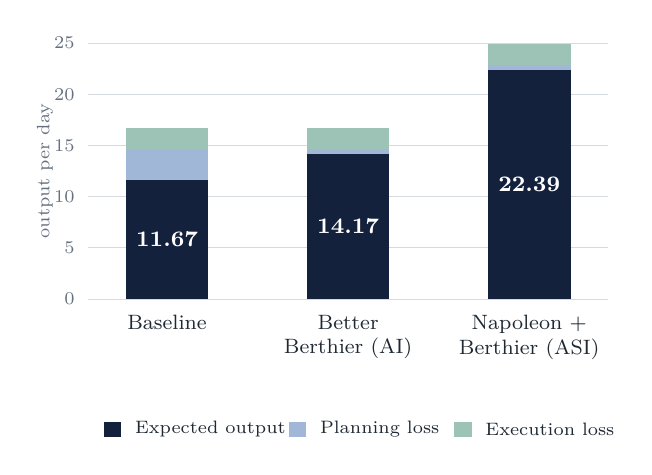
\begin{tikzpicture}[x=1cm,y=0.13cm]
      \def\bw{1.05}
      \foreach \t in {0,5,10,15,20,25}{\draw[hair,line width=0.3pt] (0,\t) -- (6.6,\t);
        \node[font=\fontsize{6.5}{7}\selectfont,text=muted,anchor=east] at (-0.05,\t) {\t};}
      \foreach \x/\net/\kb/\kl/\lab/\sub in {1.0/11.67/3.00/2.00/Baseline/{},3.3/14.17/0.50/2.00/Better/Berthier (AI),5.6/22.39/0.50/2.00/Napoleon +/Berthier (ASI)}{
        \fill[navy] (\x-\bw/2,0) rectangle (\x+\bw/2,\net);
        \fill[ber!45] (\x-\bw/2,\net) rectangle (\x+\bw/2,\net+\kb);
        \fill[lan!45] (\x-\bw/2,\net+\kb) rectangle (\x+\bw/2,\net+\kb+\kl);
        \node[font=\footnotesize\bfseries,text=white] at (\x,\net/2) {\net};
        \node[font=\fontsize{7.5}{9}\selectfont,align=center,text=ink,anchor=north] at (\x,-0.6) {\lab\\\sub};
      }
      \node[font=\fontsize{6.5}{7}\selectfont,text=muted,rotate=90] at (-0.55,12.5) {output per day};
      \begin{scope}[shift={(0.2,-13.5)},font=\fontsize{6.5}{8}\selectfont]
        \fill[navy] (0,0) rectangle (0.22,1.5); \node[anchor=west,text=ink] at (0.27,0.75) {Expected output};
        \fill[ber!45] (2.35,0) rectangle (2.57,1.5); \node[anchor=west,text=ink] at (2.62,0.75) {Planning loss};
        \fill[lan!45] (4.45,0) rectangle (4.67,1.5); \node[anchor=west,text=ink] at (4.72,0.75) {Execution loss};
      \end{scope}
    \end{tikzpicture}
    \column{0.42\textwidth}
    {\small
    \renewcommand{\arraystretch}{1.1}
    \begin{tabular}{@{}l c c c@{}}
      \toprule
      & Ideas $\lambda_A$ & Plans $\mu_B$ & Actions $\mu_L$ \\
      \midrule
      Baseline & 6 & 3 & 2 \\
      AI       & 6 & 8 & 2 \\
      ASI      & 9 & 8 & 2 \\
      \bottomrule
    \end{tabular}\par}
    \vspace{0.3cm}
    {\small Lannes completes only \textbf{two projects per day} in every scenario. Gains come from executing \emph{more valuable} projects with \emph{fewer planning errors}.\par}
    \vspace{0.25cm}
    \smallnote{Baseline: $V\sim U[0,10]$, $\kappa_B=1.5$, $\kappa_L=1$. AI: $\kappa_B=0.25$. ASI: also $V\sim U[0,14]$, $\lambda_A=9$. The top $K/\lambda_A$ share of draws is accepted. Illustrative parameters, not a forecast.}
  \end{columns}
\end{frame}

% ====================================================================== 13
\kicker{AI versus ASI}
\begin{frame}{AI and ASI act on different margins}
  \vspace{0.3cm}
  \begin{columns}[T,onlytextwidth]
    \column{0.48\textwidth}
    \begin{cardh}{\linewidth}{1.75cm}{ber}
      \cardtitle{AI \textperiodcentered{} the Berthier margin}{ber}
      \begin{itemize}\setlength{\itemsep}{2pt}
        \item Faster planning: $\tau_B\downarrow$
        \item Better planning: $\Omega_B\downarrow$
        \item Same distribution of ideas $F_A$
      \end{itemize}
    \end{cardh}
    \column{0.48\textwidth}
    \begin{cardh}{\linewidth}{1.75cm}{nap}
      \cardtitle{ASI \textperiodcentered{} also the Napoleon margin}{nap}
      \begin{itemize}\setlength{\itemsep}{2pt}
        \item More ideas: $\tau_A\downarrow$
        \item Better ideas: $F_A$ shifts up in value
        \item Retains strong planning: $\tau_B,\ \Omega_B\downarrow$
      \end{itemize}
    \end{cardh}
  \end{columns}
  \vspace{0.45cm}
  \begin{card}{\linewidth}{navy}
    \textbf{Main tension.} As long as Lannes is required, cognitive intelligence faces a physical throughput bound. Idea quality and planning accuracy still matter \emph{within} that bound.
  \end{card}
\end{frame}

% ====================================================================== 14
\kicker{Time--accuracy trade-off}
\begin{frame}{Extension: time can buy accuracy at each stage}
  \vspace{0.15cm}
  Suppose that, for one project, more time lowers each stage's expected loss:
  \[\kappa_B(t_B)=\frac{b}{t_B},\qquad \kappa_L(t_L)=\frac{\ell}{t_L},\qquad b,\ell>0.\]
  \begin{columns}[c,onlytextwidth]
    \column{0.55\textwidth}
    With a fixed time budget $T=t_B+t_L$, choose the split:
    \[\min_{t_B,t_L>0}\ \frac{b}{t_B}+\frac{\ell}{t_L}\quad\text{s.t.}\quad t_B+t_L=T\]
    \column{0.38\textwidth}
    \begin{card}{\linewidth}{ber}
      \cardtitle{Optimal split}{ber}
      \vspace{-0.3cm}
      \[\frac{t_B^*}{t_L^*}=\sqrt{\frac{b}{\ell}}\]
      \vspace{-0.15cm}
    \end{card}
  \end{columns}
  \vspace{0.25cm}
  An AI improvement that lowers $b$ cuts the planning time needed for a given accuracy.\par
  \vspace{0.12cm}
  \smallnote{In the full pipeline the optimal allocation also depends on relative stage capacity and on the value of accepted projects.}
\end{frame}

% ====================================================================== 15
\kicker{Measurement}
\begin{frame}{Lannes supplies a benchmark, not identification}
  \vspace{0.3cm}
  \begin{columns}[T,onlytextwidth]
    \column{0.4\textwidth}
    \begin{cardh}{\linewidth}{2.15cm}{lan}
      \cardtitle{What can be observed}{lan}
      \begin{itemize}\setlength{\itemsep}{2pt}
        \item Berthier's submitted plan $\hat a$
        \item Lannes's realized action $\tilde a$
        \item The realized payoff $Y$
      \end{itemize}
    \end{cardh}
    \column{0.56\textwidth}
    \begin{cardh}{\linewidth}{2.15cm}{navy}
      \cardtitle{What can be learned}{navy}
      $\tilde a-\hat a$\enspace measures execution deviation.\par\vspace{0.1cm}
      $\hat a-a^*(\xi)$\enspace measures planning deviation, \emph{if a credible benchmark optimum exists}.\par\vspace{0.1cm}
      Repeated outcomes help test whether a Napoleon's ideas were good.
    \end{cardh}
  \end{columns}
  \vspace{0.45cm}
  Physical outcomes alone do not separate poor ideas, poor plans, and execution noise. Benchmarks or additional variation are needed.
\end{frame}

% ====================================================================== 16
\kicker{Summary}
\begin{frame}{Takeaways}
  \vspace{0.1cm}
  \begin{card}{\linewidth}{navy}
    \vspace{-0.3cm}
    \[\Ycal^* \;=\; \ub{Q^*}{accepted flow}\quad\times\quad\Big(\ub{\E[V\mid V\ge z^*]}{value of selected ideas}\quad-\quad\ub{\;\kappa_B\;}{planning loss}\quad-\quad\ub{\;\kappa_L\;}{execution loss}\Big)\]
  \end{card}
  \vspace{0.2cm}
  \begin{enumerate}\setlength{\itemsep}{1pt}\small
    \item \textbf{Intelligence has distinct margins.} Conceiving, planning, and executing each have their own capacity and error.
    \item \textbf{The binding stage decides what pays.} When Lannes binds, faster planning adds nothing; only more accurate planning and better selection raise output.
    \item \textbf{Accuracy is worth the flow of projects.} Each unit of planning-loss reduction raises value by $Q^*$.
    \item \textbf{Better ideas work through selection.} More and better draws raise the quality of the $K$ projects that capacity allows.
  \end{enumerate}
\end{frame}

% ====================================================================== 17
\kicker{Next steps \textperiodcentered{} A starting point, not yet a general-equilibrium model}
\begin{frame}{Open questions for the theory}
  \vspace{0.2cm}
  \begin{enumerate}\setlength{\itemsep}{3pt}
    \item \textbf{Endogenous complexity.} Do Napoleon's most ambitious ideas need more Berthier time, more Lannes time, or carry larger error variances: $\tau_B(\xi),\ \tau_L(\xi),\ \Omega_B(\xi),\ \Omega_L(\xi)$?
    \item \textbf{Occupational choice and wages.} How does cheaper Berthier labor change demand for Napoleon-like and Lannes-like workers?
    \item \textbf{Learning and evaluation.} Can feedback from executions improve idea selection and distinguish failures of conception from failures of implementation?
  \end{enumerate}
  \vspace{0.25cm}
  \begin{card}{\linewidth}{nap}
    \textbf{Central question.} Does AI's first-order economic effect come from generating better ideas, or from making the existing stock of human ideas much easier to realize?
  \end{card}
\end{frame}

% ====================================================================== A1
\appendixtrue
\kicker{Appendix}
\begin{frame}{A1. Closed form with uniform idea values}
  \vspace{0.15cm}
  Assume $V\sim U[0,\bar v]$, constant expected losses $\kappa=\kappa_B+\kappa_L$, and downstream capacity $K$.\par
  \vspace{0.15cm}
  \begin{card}{\linewidth}{navy}
    \vspace{-0.3cm}
    \[z^*=\max\Big\{\kappa,\ \bar v\Big(1-\min\Big\{1,\tfrac{K}{\lambda_A}\Big\}\Big)\Big\}\]
    \vspace{-0.3cm}
  \end{card}\par
  \vspace{0.15cm}
  The accepted flow and its average potential value are
  \[Q^*=\lambda_A\Big(1-\frac{z^*}{\bar v}\Big),\qquad \E[V\mid V\ge z^*]=\frac{\bar v+z^*}{2},\]
  so the optimized output rate is
  \[\boxed{\;\Ycal^*=Q^*\Big(\frac{\bar v+z^*}{2}-\kappa\Big)\;}\]
\end{frame}

% ====================================================================== A2
\kicker{Appendix}
\begin{frame}{A2. Beyond independent, unbiased errors}
  \vspace{0.15cm}
  Let $\E[\varepsilon_B]=b_B$, $\E[\varepsilon_L]=b_L$, and $C_{BL}=\Cov(\varepsilon_B,\varepsilon_L)$. Then\par
  \vspace{0.15cm}
  \begin{card}{\linewidth}{navy}
    \vspace{-0.35cm}
    \begin{align*}
      \E[Y\mid\xi] = v(\xi) &- \tfrac12(b_B+b_L)^{\top}H(b_B+b_L)\\
                            &- \tfrac12\tr\!\big[H(\Omega_B+\Omega_L+C_{BL}+C_{BL}^{\top})\big]
    \end{align*}
    \vspace{-0.4cm}
  \end{card}\par
  \vspace{0.3cm}
  \begin{itemize}\setlength{\itemsep}{4pt}
    \item \textbf{Biased planning.} Berthier may systematically misunderstand Napoleon's idea.
    \item \textbf{Correlated error.} Lannes may correct, amplify, or respond to Berthier's mistakes.
    \item \textbf{Uncertain outcomes.} Additional payoff shocks leave expected output unchanged if mean-zero and independent.
  \end{itemize}
\end{frame}

\end{document}
